\documentclass[11pt]{article}
\usepackage[margin=1in]{geometry}
\usepackage{amsmath,amssymb,amsthm}
\usepackage{graphicx,booktabs,xcolor}
\usepackage[numbers]{natbib}
\usepackage{algorithm,algpseudocode}
\usepackage{placeins}
\usepackage{hyperref}
\hypersetup{colorlinks=true,linkcolor=blue!50!black,citecolor=blue!50!black,urlcolor=blue!50!black}
\newcommand{\builtdate}{9 October 2026}
\newcommand{\totalruns}{89{,}488}
\newcommand{\ncampaigns}{11}
\newcommand{\CfourHardenLowest}{142}
\newcommand{\CfourHardenSole}{16}
\newcommand{\CfourHardenSolved}{121}
\newcommand{\CfourGrowLowest}{139}
\newcommand{\CfourGrowSole}{11}
\newcommand{\CfourGrowSolved}{119}
\newcommand{\CfourRigidLowest}{155}
\newcommand{\CfourRigidSole}{23}
\newcommand{\CfourRigidSolved}{132}
\newcommand{\CfourSaLowest}{72}
\newcommand{\CfourSaSole}{2}
\newcommand{\CfourSaSolved}{69}
\newcommand{\CfourPcLowest}{64}
\newcommand{\CfourPcSole}{0}
\newcommand{\CfourPcSolved}{63}
\newcommand{\CfourSignGrow}{11 vs 9}
\newcommand{\CfourSignPGrow}{0.41}
\newcommand{\CfourSignRigid}{7 vs 18}
\newcommand{\CfourSignPRigid}{0.022}
\newcommand{\CfourSignSa}{57 vs 5}
\newcommand{\CfourSignPSa}{1.5e-12}
\newcommand{\CfourSignPc}{59 vs 1}
\newcommand{\CfourSignPPc}{5.3e-17}
\newcommand{\CfourInstances}{188}
\newcommand{\CfourUnsolved}{46}
\newcommand{\CfourSquInSquHardenLowest}{28}
\newcommand{\CfourSquInSquHardenSole}{7}
\newcommand{\CfourSquInSquRigidLowest}{20}
\newcommand{\CfourSquInSquRigidSole}{0}
\newcommand{\CfourSquInSquGrowLowest}{21}
\newcommand{\CfourSquInSquGrowSole}{0}
\newcommand{\CfourSquInSquN}{28}
\newcommand{\CfourSquInCirHardenLowest}{16}
\newcommand{\CfourSquInCirHardenSole}{7}
\newcommand{\CfourSquInCirRigidLowest}{19}
\newcommand{\CfourSquInCirRigidSole}{9}
\newcommand{\CfourSquInCirGrowLowest}{11}
\newcommand{\CfourSquInCirGrowSole}{2}
\newcommand{\CfourSquInCirN}{28}
\newcommand{\CfourSquInTriHardenLowest}{27}
\newcommand{\CfourSquInTriHardenSole}{0}
\newcommand{\CfourSquInTriRigidLowest}{29}
\newcommand{\CfourSquInTriRigidSole}{1}
\newcommand{\CfourSquInTriGrowLowest}{24}
\newcommand{\CfourSquInTriGrowSole}{0}
\newcommand{\CfourSquInTriN}{29}
\newcommand{\CfourTriInTriHardenLowest}{19}
\newcommand{\CfourTriInTriHardenSole}{1}
\newcommand{\CfourTriInTriRigidLowest}{24}
\newcommand{\CfourTriInTriRigidSole}{4}
\newcommand{\CfourTriInTriGrowLowest}{22}
\newcommand{\CfourTriInTriGrowSole}{3}
\newcommand{\CfourTriInTriN}{28}
\newcommand{\CfourTriInSquHardenLowest}{10}
\newcommand{\CfourTriInSquHardenSole}{1}
\newcommand{\CfourTriInSquRigidLowest}{18}
\newcommand{\CfourTriInSquRigidSole}{7}
\newcommand{\CfourTriInSquGrowLowest}{19}
\newcommand{\CfourTriInSquGrowSole}{5}
\newcommand{\CfourTriInSquN}{28}
\newcommand{\CfourHexInSquHardenLowest}{15}
\newcommand{\CfourHexInSquHardenSole}{0}
\newcommand{\CfourHexInSquRigidLowest}{17}
\newcommand{\CfourHexInSquRigidSole}{2}
\newcommand{\CfourHexInSquGrowLowest}{15}
\newcommand{\CfourHexInSquGrowSole}{1}
\newcommand{\CfourHexInSquN}{18}
\newcommand{\CfourCirInSquHardenLowest}{27}
\newcommand{\CfourCirInSquHardenSole}{0}
\newcommand{\CfourCirInSquRigidLowest}{28}
\newcommand{\CfourCirInSquRigidSole}{0}
\newcommand{\CfourCirInSquGrowLowest}{27}
\newcommand{\CfourCirInSquGrowSole}{0}
\newcommand{\CfourCirInSquN}{29}
\newcommand{\CsevenHardenLowest}{142}
\newcommand{\CsevenHardenSole}{13}
\newcommand{\CsevenHardenSolved}{125}
\newcommand{\CsevenGrowLowest}{144}
\newcommand{\CsevenGrowSole}{9}
\newcommand{\CsevenGrowSolved}{129}
\newcommand{\CsevenRigidLowest}{155}
\newcommand{\CsevenRigidSole}{16}
\newcommand{\CsevenRigidSolved}{133}
\newcommand{\CsevenSaLowest}{125}
\newcommand{\CsevenSaSole}{6}
\newcommand{\CsevenSaSolved}{115}
\newcommand{\CsevenPcLowest}{72}
\newcommand{\CsevenPcSole}{1}
\newcommand{\CsevenPcSolved}{71}
\newcommand{\CsevenSignGrow}{9 vs 13}
\newcommand{\CsevenSignPGrow}{0.26}
\newcommand{\CsevenSignRigid}{6 vs 14}
\newcommand{\CsevenSignPRigid}{0.058}
\newcommand{\CsevenSignSa}{21 vs 11}
\newcommand{\CsevenSignPSa}{0.055}
\newcommand{\CsevenSignPc}{59 vs 5}
\newcommand{\CsevenSignPPc}{4.5e-13}
\newcommand{\CsevenInstances}{188}
\newcommand{\CsevenUnsolved}{43}
\newcommand{\CsevenSquInSquHardenLowest}{27}
\newcommand{\CsevenSquInSquHardenSole}{5}
\newcommand{\CsevenSquInSquRigidLowest}{23}
\newcommand{\CsevenSquInSquRigidSole}{1}
\newcommand{\CsevenSquInSquGrowLowest}{21}
\newcommand{\CsevenSquInSquGrowSole}{0}
\newcommand{\CsevenSquInSquN}{28}
\newcommand{\CsevenSquInCirHardenLowest}{16}
\newcommand{\CsevenSquInCirHardenSole}{6}
\newcommand{\CsevenSquInCirRigidLowest}{15}
\newcommand{\CsevenSquInCirRigidSole}{3}
\newcommand{\CsevenSquInCirGrowLowest}{17}
\newcommand{\CsevenSquInCirGrowSole}{4}
\newcommand{\CsevenSquInCirN}{28}
\newcommand{\CsevenSquInTriHardenLowest}{28}
\newcommand{\CsevenSquInTriHardenSole}{0}
\newcommand{\CsevenSquInTriRigidLowest}{29}
\newcommand{\CsevenSquInTriRigidSole}{0}
\newcommand{\CsevenSquInTriGrowLowest}{27}
\newcommand{\CsevenSquInTriGrowSole}{0}
\newcommand{\CsevenSquInTriN}{29}
\newcommand{\CsevenTriInTriHardenLowest}{18}
\newcommand{\CsevenTriInTriHardenSole}{0}
\newcommand{\CsevenTriInTriRigidLowest}{26}
\newcommand{\CsevenTriInTriRigidSole}{4}
\newcommand{\CsevenTriInTriGrowLowest}{24}
\newcommand{\CsevenTriInTriGrowSole}{2}
\newcommand{\CsevenTriInTriN}{28}
\newcommand{\CsevenTriInSquHardenLowest}{14}
\newcommand{\CsevenTriInSquHardenSole}{2}
\newcommand{\CsevenTriInSquRigidLowest}{22}
\newcommand{\CsevenTriInSquRigidSole}{7}
\newcommand{\CsevenTriInSquGrowLowest}{17}
\newcommand{\CsevenTriInSquGrowSole}{3}
\newcommand{\CsevenTriInSquN}{28}
\newcommand{\CsevenHexInSquHardenLowest}{15}
\newcommand{\CsevenHexInSquHardenSole}{0}
\newcommand{\CsevenHexInSquRigidLowest}{16}
\newcommand{\CsevenHexInSquRigidSole}{1}
\newcommand{\CsevenHexInSquGrowLowest}{14}
\newcommand{\CsevenHexInSquGrowSole}{0}
\newcommand{\CsevenHexInSquN}{18}
\newcommand{\CsevenCirInSquHardenLowest}{24}
\newcommand{\CsevenCirInSquHardenSole}{0}
\newcommand{\CsevenCirInSquRigidLowest}{24}
\newcommand{\CsevenCirInSquRigidSole}{0}
\newcommand{\CsevenCirInSquGrowLowest}{24}
\newcommand{\CsevenCirInSquGrowSole}{0}
\newcommand{\CsevenCirInSquN}{29}
\newcommand{\CubesHardenTwelve}{2.942809}
\newcommand{\CubesRigidTwelve}{3.000000}
\newcommand{\CubesGrowTwelve}{2.947506}
\newcommand{\CubesBelow}{none}
\newcommand{\CtauOne}{7}
\newcommand{\CtauHalf}{15}
\newcommand{\CtauQuarter}{18}
\newcommand{\CtauZero}{17}
\newcommand{\CtauN}{40}
\newcommand{\CtauSquares}{3, 4, 2, 0}
\newcommand{\CtauTriangles}{2, 7, 8, 10}
\newcommand{\CbudgetOneHarden}{3}\newcommand{\CbudgetOneRigid}{17}
\newcommand{\CbudgetThreeHarden}{5}\newcommand{\CbudgetThreeRigid}{16}
\newcommand{\CbudgetTenHarden}{9}\newcommand{\CbudgetTenRigid}{16}
\newcommand{\CbudgetN}{20}
\newcommand{\PortRigidSixtyFour}{138}
\newcommand{\PortRigidHarden}{139}
\newcommand{\PortRigidGrow}{137}
\newcommand{\PortSign}{4 vs 3}
\newcommand{\PortP}{0.5}

\newcommand{\BootHarden}{126--140}
\newcommand{\BootGrow}{123--138}
\newcommand{\BootRigid}{139--153}
\newcommand{\BootSa}{89--107}
\newcommand{\BootPc}{40--56}
\newcommand{\BootDRH}{3 to 24}
\newcommand{\BootDRHMed}{14}
\newcommand{\BootDRHPos}{99\%}
\newcommand{\BootDRG}{5 to 27}
\newcommand{\BootDRGMed}{16}
\newcommand{\BootDRGPos}{99\%}
\newcommand{\BootDGH}{-13 to 9}
\newcommand{\BootDGHMed}{-2}
\newcommand{\BootDGHPos}{30\%}
\newcommand{\EligHarden}{97\%}
\newcommand{\EligGrow}{98\%}
\newcommand{\EligRigid}{100\%}
\newcommand{\EligSa}{94\%}
\newcommand{\EligPc}{56\%}
\newcommand{\RangeSmallHarden}{54}
\newcommand{\RangeSmallGrow}{54}
\newcommand{\RangeSmallRigid}{56}
\newcommand{\RangeSmallSa}{56}
\newcommand{\RangeSmallPc}{47}
\newcommand{\RangeSmallN}{58}
\newcommand{\RangeMidHarden}{50}
\newcommand{\RangeMidGrow}{57}
\newcommand{\RangeMidRigid}{52}
\newcommand{\RangeMidSa}{43}
\newcommand{\RangeMidPc}{20}
\newcommand{\RangeMidN}{70}
\newcommand{\RangeLargeHarden}{38}
\newcommand{\RangeLargeGrow}{33}
\newcommand{\RangeLargeRigid}{47}
\newcommand{\RangeLargeSa}{26}
\newcommand{\RangeLargePc}{5}
\newcommand{\RangeLargeN}{60}
\newcommand{\StepsGrowTwenty}{11{,}500}
\newcommand{\StepsGrowThirty}{11{,}500}
\newcommand{\StepsHardenTwenty}{11{,}500}
\newcommand{\StepsHardenThirty}{11{,}500}
\newcommand{\StepsPcTwenty}{19{,}148}
\newcommand{\StepsPcThirty}{20{,}530}
\newcommand{\StepsRigidTwenty}{11{,}500}
\newcommand{\StepsRigidThirty}{11{,}500}
\newcommand{\StepsSaTwenty}{66{,}854}
\newcommand{\StepsSaThirty}{104{,}043}

\newcommand{\SnapHLower}{17}
\newcommand{\SnapXLower}{36}
\newcommand{\SnapTies}{135}
\newcommand{\SnapP}{0.013}
\newcommand{\SnapHOnly}{6}
\newcommand{\SnapXOnly}{16}
\newcommand{\SnapPReached}{0.052}
\newcommand{\SnapRXLower}{20}
\newcommand{\SnapRRLower}{20}
\newcommand{\SnapRP}{1}
\newcommand{\SnapSquSqu}{6--0}
\newcommand{\SnapRSquSqu}{1--2}
\newcommand{\SnapSquCir}{5--11}
\newcommand{\SnapRSquCir}{10--6}
\newcommand{\SnapSquTri}{0--1}
\newcommand{\SnapRSquTri}{0--0}
\newcommand{\SnapTriTri}{0--8}
\newcommand{\SnapRTriTri}{0--2}
\newcommand{\SnapTriSqu}{6--14}
\newcommand{\SnapRTriSqu}{8--9}
\newcommand{\SnapHexSqu}{0--2}
\newcommand{\SnapRHexSqu}{1--1}
\newcommand{\SnapCirSqu}{0--0}
\newcommand{\SnapRCirSqu}{0--0}
\newcommand{\AreaHLower}{20}
\newcommand{\AreaXLower}{31}
\newcommand{\AreaTies}{137}
\newcommand{\AreaP}{0.16}
\newcommand{\AreaHOnly}{6}
\newcommand{\AreaXOnly}{15}
\newcommand{\AreaPReached}{0.078}
\newcommand{\AreaRXLower}{15}
\newcommand{\AreaRRLower}{14}
\newcommand{\AreaRP}{1}
\newcommand{\AreaSquSqu}{5--1}
\newcommand{\AreaRSquSqu}{2--1}
\newcommand{\AreaSquCir}{9--8}
\newcommand{\AreaRSquCir}{8--4}
\newcommand{\AreaSquTri}{0--1}
\newcommand{\AreaRSquTri}{0--0}
\newcommand{\AreaTriTri}{1--8}
\newcommand{\AreaRTriTri}{0--3}
\newcommand{\AreaTriSqu}{5--11}
\newcommand{\AreaRTriSqu}{5--6}
\newcommand{\AreaHexSqu}{0--2}
\newcommand{\AreaRHexSqu}{0--0}
\newcommand{\AreaCirSqu}{0--0}
\newcommand{\AreaRCirSqu}{0--0}
\newcommand{\BatN}{28}
\newcommand{\BatHReached}{49}
\newcommand{\BatHAll}{14}
\newcommand{\BatHSome}{4}
\newcommand{\BatRReached}{46}
\newcommand{\BatRAll}{14}
\newcommand{\BatRSome}{2}
\newcommand{\BatSqElevenH}{2}
\newcommand{\BatSqElevenR}{0}
\newcommand{\BatSqTwentyNineH}{2}
\newcommand{\BatSqTwentyNineR}{0}
\newcommand{\BatTriTwentyNineH}{1}
\newcommand{\BatTriTwentyNineR}{3}
\newcommand{\LongN}{14}
\newcommand{\LongHardenLowest}{13}
\newcommand{\LongHardenSole}{5}
\newcommand{\LongHardenReached}{12}
\newcommand{\LongGrowLowest}{7}
\newcommand{\LongGrowSole}{0}
\newcommand{\LongGrowReached}{7}
\newcommand{\LongRigidLowest}{8}
\newcommand{\LongRigidSole}{0}
\newcommand{\LongRigidReached}{8}
\newcommand{\LongSaLowest}{9}
\newcommand{\LongSaSole}{1}
\newcommand{\LongSaReached}{9}
\newcommand{\LongPcLowest}{6}
\newcommand{\LongPcSole}{0}
\newcommand{\LongPcReached}{6}
\newcommand{\LongHLower}{6}
\newcommand{\LongRLower}{0}
\newcommand{\LongP}{0.031}
\newcommand{\LongHardenSoleNs}{17, 19, 26, 28, 29}
\newcommand{\LongHardenOnlyReachedNs}{17, 19, 26, 29}
\newcommand{\LongSaOnlyReachedNs}{27}
\newcommand{\LongBelow}{0}
\newcommand{\BudOneH}{7}
\newcommand{\BudOneR}{2}
\newcommand{\BudOneP}{0.18}
\newcommand{\BudOneHReached}{17}
\newcommand{\BudOneRReached}{15}
\newcommand{\BudThreeH}{4}
\newcommand{\BudThreeR}{3}
\newcommand{\BudThreeP}{1}
\newcommand{\BudThreeHReached}{18}
\newcommand{\BudThreeRReached}{16}
\newcommand{\BudMoreH}{6}
\newcommand{\BudMoreR}{2}
\newcommand{\BudMoreP}{0.29}
\newcommand{\BudMoreHReached}{18}
\newcommand{\BudMoreRReached}{16}
\newcommand{\BudLvMLH}{3}
\newcommand{\BudLvMMH}{3}
\newcommand{\BudLMPH}{1}
\newcommand{\BudGainH}{4}
\newcommand{\BudLossH}{3}
\newcommand{\BudLvMLR}{3}
\newcommand{\BudLvMMR}{2}
\newcommand{\BudLMPR}{1}
\newcommand{\BudGainR}{5}
\newcommand{\BudLossR}{0}
\newcommand{\BudN}{28}

\IfFileExists{decision.tex}{\newcommand{\DecN}{60}
\newcommand{\DecPilotLower}{2}
\newcommand{\DecRigidLower}{3}
\newcommand{\DecTies}{55}
\newcommand{\DecP}{1}
\newcommand{\DecHLower}{3}
\newcommand{\DecHRLower}{17}
\newcommand{\DecHP}{0.0026}
\newcommand{\DecPicked}{20}
\newcommand{\DecReachedRigid}{40}
\newcommand{\DecReachedHarden}{32}
\newcommand{\DecReachedPilot}{41}
\newcommand{\DecTPicked}{3}
\newcommand{\DecTChanged}{17}
\newcommand{\DecTLower}{2}
\newcommand{\DecTRLower}{3}
}{}
\IfFileExists{refine.tex}{\newcommand{\RefN}{28}
\newcommand{\RefRawHarden}{6}
\newcommand{\RefRawGrow}{19}
\newcommand{\RefRawRigid}{3}
\newcommand{\RefRawSa}{1}
\newcommand{\RefRawPc}{0}
\newcommand{\RefEqHarden}{23}
\newcommand{\RefEqGrow}{20}
\newcommand{\RefEqRigid}{19}
\newcommand{\RefEqSa}{17}
\newcommand{\RefEqPc}{4}
\newcommand{\RefPolHarden}{24}
\newcommand{\RefPolGrow}{20}
\newcommand{\RefPolRigid}{18}
\newcommand{\RefPolSa}{14}
\newcommand{\RefPolPc}{2}
}{}
\newcommand{\MechSquSquHardenMove}{0.45}
\newcommand{\MechSquSquHardenTurn}{23}
\newcommand{\MechSquSquHardenTilt}{0.13}
\newcommand{\MechSquSquHardenOrder}{0.53}
\newcommand{\MechSquSquRigidMove}{0.36}
\newcommand{\MechSquSquRigidTurn}{5}
\newcommand{\MechSquSquRigidTilt}{0.11}
\newcommand{\MechSquSquRigidOrder}{0.81}
\newcommand{\MechSquCirHardenMove}{0.52}
\newcommand{\MechSquCirHardenTurn}{21}
\newcommand{\MechSquCirHardenOrder}{0.24}
\newcommand{\MechSquCirRigidMove}{0.43}
\newcommand{\MechSquCirRigidTurn}{22}
\newcommand{\MechSquCirRigidOrder}{0.37}
\newcommand{\MechSquTriHardenMove}{0.35}
\newcommand{\MechSquTriHardenTurn}{23}
\newcommand{\MechSquTriHardenTilt}{0.06}
\newcommand{\MechSquTriHardenOrder}{0.29}
\newcommand{\MechSquTriRigidMove}{0.17}
\newcommand{\MechSquTriRigidTurn}{9}
\newcommand{\MechSquTriRigidTilt}{0.03}
\newcommand{\MechSquTriRigidOrder}{0.20}
\newcommand{\MechTriTriHardenMove}{0.53}
\newcommand{\MechTriTriHardenTurn}{30}
\newcommand{\MechTriTriHardenTilt}{0.00}
\newcommand{\MechTriTriHardenOrder}{0.28}
\newcommand{\MechTriTriRigidMove}{0.28}
\newcommand{\MechTriTriRigidTurn}{18}
\newcommand{\MechTriTriRigidTilt}{0.00}
\newcommand{\MechTriTriRigidOrder}{0.23}
\newcommand{\MechTriSquHardenMove}{0.62}
\newcommand{\MechTriSquHardenTurn}{28}
\newcommand{\MechTriSquHardenTilt}{0.29}
\newcommand{\MechTriSquHardenOrder}{0.10}
\newcommand{\MechTriSquRigidMove}{0.45}
\newcommand{\MechTriSquRigidTurn}{26}
\newcommand{\MechTriSquRigidTilt}{0.21}
\newcommand{\MechTriSquRigidOrder}{0.06}
\newcommand{\MechHexSquHardenMove}{0.13}
\newcommand{\MechHexSquHardenTurn}{15}
\newcommand{\MechHexSquHardenTilt}{0.07}
\newcommand{\MechHexSquHardenOrder}{0.44}
\newcommand{\MechHexSquRigidMove}{0.11}
\newcommand{\MechHexSquRigidTurn}{7}
\newcommand{\MechHexSquRigidTilt}{0.00}
\newcommand{\MechHexSquRigidOrder}{0.71}
\newcommand{\MechSoleN}{5}
\newcommand{\MechSoleTiltH}{0.45}
\newcommand{\MechSoleTiltR}{0.28}
\newcommand{\MechSoleMore}{5}
\newcommand{\MechTriFailN}{4}
\newcommand{\MechTriFailMoveH}{0.54}
\newcommand{\MechTriFailMoveR}{0.30}


\title{Soft-to-Rigid: Shape Continuation as an Alternative Search\\ for Packing Congruent Shapes}
\author{Yohei Nakajima\thanks{Experiments, code and verification were developed with the assistance of Claude (Anthropic); see the acknowledgements.}}
\date{\builtdate}

\begin{document}
\maketitle

\begin{abstract}
Searches for dense packings of congruent shapes move rigid pieces. Hardening starts each piece as its inscribed disk and rounds it into the real shape while the container is compressed. We ask whether it is a search worth running alongside existing ones, and test it at matched budget and comparable tuning against rigid starts, growth, simulated annealing and perturbation--compression on seven families of squares, triangles, hexagons and disks in squares, triangles and circles (\CsevenInstances{} instances), scoring each method by the lowest container size it reaches. Hardening is not a better default: tuned rigid starts reach the lowest size most often. It is a different search. On squares in a square it reaches packings the other four methods miss, including Trump's $n=11$ and Wainwright's $n=19$ in 32 runs per method, and in a later confirmatory campaign at ten times the budget (16 runs per method) the only one to reach the best known packings for $n=\LongHardenOnlyReachedNewNs$, where annealing alone reaches $n=\LongSaOnlyReachedNs$. In exploratory ablations, compressing disks and then switching to polygons at once, or growing rigid polygons along hardening's area schedule, shows no detectable difference from rigid starts, and hardening's unique packings contain more tilted pieces. The bias costs elsewhere: hardening is worse on triangles and on four families held out from all development, where a short pilot that chooses the path per instance does no better than always starting rigid. Shape continuation is an alternative search that reaches different packings, worth keeping beside rigid ones; we did not show that splitting a fixed budget between them pays, and we have no test that predicts where it helps. Every experiment was planned before it ran, every run is replayable, and every number is generated from an event log.

\end{abstract}

\section{Introduction}
How small a container holds $n$ copies of a given shape? For unit squares in a square the question goes back to Erd\H{o}s and Graham \cite{erdosgraham}; catalogues now cover squares, triangles, hexagons and cubes in squares, triangles, circles and cubes \cite{friedmancenter,squaresproject}, and most entries are best known packings found by search rather than proved optimal. Most searches move rigid pieces: simulated annealing \cite{kirkpatrick}, perturbation and compression \cite{Gensane2004,gensane}, growing the pieces in size \cite{lubachevsky}, overlap minimisation in a shrinking container \cite{Umetani2009,Gardeyn2025}, or global solvers on exact non-overlap models \cite{Berthold2026}.

This paper changes the pieces instead. \emph{Hardening} starts every piece as the disk inscribed in it, compresses the disks under inward pressure on the container, and deforms them into the real shape while the pressure continues. It is graduated non-convexity \cite{blake} applied to geometry: a disk has no orientation, so the pieces are already densely packed when their corners appear and rotation becomes a choice. The shape family it moves along, a polygon dilated by a disk at fixed inradius, is not new: it is the spheropolygon of discrete-element modelling \cite{AlonsoMarroquin2008}, and Jin, Lu and Li moved dense periodic packings along its 3D analogue between tetrahedra and spheres \cite{Jin2015}. Jin, Lu and Li also ran it from spheres toward tetrahedra, in periodic packings. What we have not found is its use as an optimisation path toward a prescribed polygon inside a finite container, evaluated against tuned rigid searches for best known packings (Section~\ref{sec:related}). On squares it recovers several classical packings from random starts, and in 3D it found a packing of 12 unit cubes in a cube smaller than the best known one \cite{nakajima12}.

Here we ask whether that is a property of the path or of the problems we tried. We compare three paths through shape space (hardening, growing, and rigid pieces on the same schedule) and two classical baselines on seven families of shapes and containers (\totalruns{} runs in \ncampaigns{} campaigns), with matched budgets and comparable tuning effort. Since a packing search is judged by the best packing it ever finds, the comparison is by the \emph{lowest} container size each method reaches in a fixed number of runs, after constrained numerical tightening; the procedure being compared is the batch of runs, not a single run \cite{Birattari2005}. Our findings:
\begin{itemize}\itemsep1pt
\item No path is best everywhere. Untuned, hardening looked better than rigid starts; tuned with comparable effort, rigid starts on the same schedule reach the lowest size most often (Table~\ref{tab:main}).
\item Which path wins depends on the family. For squares in a square, hardening reaches the lowest size on \CsevenSquInSquHardenLowest{} of \CsevenSquInSquN{} instances and is the only method that low on \CsevenSquInSquHardenSole, including Trump's $n=11$ and Wainwright's $n=19$ packings; for triangles, rigid or growing starts are better (Section~\ref{sec:learned}).
\item Neither the disk-compressed start nor the area schedule alone reproduces this pattern (Table~\ref{tab:ablate}), and hardening's unique square packings end with more tilted pieces than rigid starts' best (Figure~\ref{fig:mechanism}). The pre-registered tests of these ablations are inconclusive on squares in a square.
\item On four families held out from all development, hardening is worse than rigid starts, and a pilot that chooses the path per instance is no better than always starting rigid (Table~\ref{tab:decision}).
\item An earlier indication that hardening gains more from longer runs did not replicate.
\end{itemize}
The result is a negative one with a specific exception, and the paper reports it as such. The study's other contribution is its record: every experiment was planned in writing before it ran, every run can be replayed, and every number in this paper is generated from an event log. Section~\ref{sec:matters} discusses where shape continuation could be useful beyond record tables.

\section{Related work}\label{sec:related}
\paragraph{Changing shape during a packing simulation.} Hard-particle physics has long changed particle shape during a run. The event-driven molecular dynamics of Donev, Torquato and Stillinger \cite{Donev2005a}, which generalises Lubachevsky--Stillinger growth \cite{lubachevsky}, explicitly allows time-dependent particle shapes. ``Digital alchemy'' \cite{vanAnders2015,Geng2019} treats shape parameters as thermodynamic variables sampled by Monte Carlo shape moves, to design shapes for a target structure. Closest to our parametrisation, Jin, Lu and Li \cite{Jin2015} take spherotetrahedra (a tetrahedron dilated by a ball, with a roundness ratio defined relative to a tetrahedron of the same inscribed sphere) and evolve dense periodic packings by gradually increasing the roundness from tetrahedron toward sphere. Superdisk and superball families \cite{Jiao2008,Jiao2009}, truncation families \cite{Engel2012} and rounded cubes in spherical confinement \cite{Wang2018} interpolate between round and faceted shapes, but packings are computed separately at each shape. Minkowski rounding is standard in discrete-element modelling as spheropolygons \cite{AlonsoMarroquin2008,GalindoTorres2010}, where it smooths contact geometry but is held fixed. Hardening uses the same inradius-preserving family, runs it from disk to polygon, and uses it as an optimisation homotopy toward a prescribed shape in a finite container. It is an instance of graduated non-convexity and continuation \cite{blake,AllgowerGeorg1990}, for which there is theory on when following a path beats a cold start and when it need not \cite{Mobahi2015,Hazan2016}.

\paragraph{Disks as a stand-in for polygons.} In operations research, inscribed circles appear as relaxations or surrogates: QP-Nest \cite{Jones2014} bounds nesting problems by enforcing non-overlap only on inscribed circles, and sparrow \cite{Gardeyn2025} builds its overlap proxy from inscribed ``poles''. In facility layout and floorplanning, modules are first modelled as circles and then converted to exact shapes in a second stage \cite{AnjosVannelli2002,Luo2008}. These use circles as a fixed surrogate or as a one-shot initial solution. We deform each piece continuously from its inscribed disk while the container is compressed, and test separately whether the disk-compressed start or the gradual path is responsible for any effect (campaign C11).

\paragraph{Packing in containers.} Phi-functions \cite{Bennell2010,Romanova2018} and separating-line programs \cite{Peralta2018} give exact non-overlap models; our tightening step is a separating-line program of this kind. Overlap minimisation in a shrinking container dominates irregular strip packing \cite{Umetani2009,Imamichi2009,Egeblad2007,Gardeyn2025}, with jostling as a constructive alternative \cite{Dowsland1998}; analytical placers replace overlap with a smooth density penalty of increasing weight \cite{Lu2015}; and gradient descent on poses with an adaptively shrinking container has recently been applied to irregular 3D objects \cite{Gupta2026}. Our energy is of this family; what differs is that the pieces' shapes change along the way.

\paragraph{Records.} Best known packings of equal pieces come from Friedman's survey and Packing Center \cite{friedmansurvey,friedmancenter}, the Squares Project \cite{squaresproject} and Packomania \cite{packomania}. Record-finding methods include billiards and growth \cite{lubachevsky,LubachevskyGraham1997}, perturbation--compression \cite{Gensane2004,gensane}, perturbation-based thresholding search \cite{Lai2023}, periodic adaptive-shrinking-cell and divide-and-concur optimisation \cite{TorquatoJiao2009,Kallus2010}, global MINLP solvers \cite{Berthold2026}, and LLM-driven program search \cite{Novikov2025,Georgiev2025,hyra}. Berthold et al.\ \cite{Berthold2026} solve regular polygons in regular polygons and Platonic solids in Platonic solids for $n\le30$; their supplement lists 12 cubes at $2.94281$ (Friedman's 1998 value), and Hyra \cite{hyra} later reports $2.93277$. Records for squares in a square at larger $n$ ($n\ge88$) continue to fall to an iterative ``shrink-hopping'' search with exact certificates \cite{squish}.

\paragraph{Evaluating stochastic searches.} We report each method's lowest value over a fixed number of runs, with best-of-$k$ curves and resampling intervals, following the argument that a search is used for its best result \cite{Birattari2005} and in the spirit of performance profiles and time-to-target plots \cite{Dolan2002,Aiex2007,Hansen2021}. Lai et al.\ \cite{Lai2023} report best, mean and success rate over 20 runs against Packomania; we add matched budgets, matched tuning effort and pre-registered decision rules.

\section{Method}\label{sec:method}
\paragraph{Pieces and paths.} A piece is a regular polygon $P$ with unit side and inradius $\rho$ (a unit square, triangle or hexagon), or a unit-diameter disk. Its \emph{shape state} is
\[
P(\gamma,\tau)=\gamma\big[(1-\tau)\,P\;\oplus\;\tau\rho\,D\big],
\]
the polygon scaled about its incenter, dilated by a disk of radius $\tau\rho$, and scaled by $\gamma$. At $\tau=1$ it is the inscribed disk, at $\tau=0$ the polygon, and for $\gamma\le1$ every state lies inside the polygon, so moving toward $(\gamma,\tau)=(1,0)$ only grows the piece. A \emph{path} is a schedule for $(\gamma,\tau)$:
\begin{itemize}\itemsep0pt
\item \textbf{harden}: $\gamma=1$, $\tau:1\to0$ (disks harden into polygons);
\item \textbf{grow}: $\tau=0$, $\gamma:\gamma_0\to1$ (rigid polygons grow, as in Lubachevsky--Stillinger \cite{lubachevsky});
\item \textbf{rigid}: $(\gamma,\tau)=(1,0)$ throughout, with the same schedule;
\end{itemize}
plus two classical baselines on rigid pieces: \textbf{sa}, Metropolis simulated annealing over poses and container size \cite{kirkpatrick}, and \textbf{pc}, perturbation--compression \cite{gensane} (shrink, relax, perturb on failure).

\paragraph{Energy.} The container (square, equilateral triangle or circle) is centred at the origin with size $L$. For poses $(x_i,y_i,\theta_i)$,
\[
E=\sum_{i<j}\big(2r-\operatorname{sd}_{ij}\big)_+^2+\sum_{i}\sum_{v}\big(\text{wall violation of }v\big)_+^2+\mu L,
\]
where $r=\gamma\tau\rho$, $\operatorname{sd}_{ij}$ is the signed distance between the cores (exact vertex--edge distance when apart, minus the separating-axis penetration depth when overlapping) and $v$ ranges over core vertices. The term $\mu L$ is inward pressure. Positions, angles and $L$ follow momentum gradient descent with analytic gradients (checked against finite differences, relative error below $10^{-7}$ on $1.7\times10^4$ components) and decaying Gaussian noise. A run compresses at pressure $3\mu$, follows its path while $L$ settles under pressure $\mu$, then lets $\mu$ decay with rigid pieces. In 3D the same holds for cubes with quaternion orientations \cite{nakajima12}.

\paragraph{From a run to a certified packing.} Penalties tolerate small overlaps, so every run is \emph{legalised}: centres are scaled apart about their mean until no pair overlaps by more than $10^{-12}$ under the separating-axis test, and the smallest container (translation free) is measured. Near-best runs are then \emph{tightened}: minimise $L$ over poses and one separating line (plane) per nearby pair, with every vertex inside the container, by SLSQP in trust-region outer iterations, keeping a step only if the independently legalised size decreases. A tightened packing below a catalogue value is spread to a clearance of $10^{-6}$ and checked twice: in floating point and in exact rational arithmetic (rational rotations from $\tan(\theta/2)$, pieces inflated by $10^{-8}$, an explicit rational separating direction for every pair).

\paragraph{Fair comparison.} All five methods are given the same number of pair evaluations per run (that of a \textbf{harden} run at the same $n$) and comparable tuning: $3\times3$ grids over their two main parameters on held-out instances, with fixed scoring rules (Section~\ref{sec:breadth}).

\section{From squares to cubes}\label{sec:story}
The method was developed on unit squares in a square, where records are dense and audited \cite{squaresproject,friedmansurvey}. With the original schedule, hardening reaches Trump's packing for $n=11$ \cite{trump} (now proved optimal \cite{squaresproject}) in 4 of 80 random starts at three times the base budget (1 of 80 at the base budget), and tightening takes them to the record within $10^{-14}$; rigid starts with the same schedule reach it in none of 80 at either budget (campaign C00).

The same method in 3D, with quaternion orientations and the 15-axis separating test, found a packing of 12 unit cubes in a cube of side $2.9315185$, below the previous best known $2.9327718$ \cite{hyra,nakajima12}, which had itself improved Friedman's 1998 value $2.94281$ (the value the global solvers of Berthold et al.\ \cite{Berthold2026} also reach). Campaign C05 repeats the cube experiment with three gradient paths and two settings at the record's budget (Table~\ref{tab:cubes}). Hardening has the lowest side of the three paths at $n=11$, 12 and 13 under both settings, all paths reach Friedman's $n=9$ packing, and with tuned settings hardening and rigid starts also reach his $n=10$ packing $2+1/\sqrt2$, which the original schedule never did. Rigid starts end at the trivial side 3 for $n\ge12$. In these 32 seeds nothing went below a catalogue value: the best side at $n=12$ is \CubesHardenTwelve{} (grow \CubesGrowTwelve, rigid \CubesRigidTwelve), while the record came from one of 192 runs. At $n=13$ hardening reaches $2.956145$, consistent with Friedman's $2.956+$ to the precision printed.

\begin{table}[t]\centering\small
\begin{tabular}{rrrrrrrr}
\toprule
 & & \multicolumn{3}{c}{original settings} & \multicolumn{3}{c}{2D-tuned settings}\\
$n$ & best known & harden & grow & rigid & harden & grow & rigid\\
\midrule
9 & 2.70711 & \textbf{2.70711} & \textbf{2.70711} & \textbf{2.70711} & \textbf{2.70711} & \textbf{2.70711} & \textbf{2.70711}\\
10 & 2.70711 & 2.76777 & 2.76777 & 2.89443 & \textbf{2.70711} & 2.76777 & \textbf{2.70711}\\
11 & 2.88295 & \textbf{2.89443} & 2.91739 & 2.91899 & 2.91250 & 2.91328 & 2.94281\\
12 & 2.93277 & 2.94301 & 2.98587 & 3.00000 & \textbf{2.94281} & 2.94751 & 3.00000\\
13 & 2.95600 & 2.99497 & 3.00000 & 3.00000 & \textbf{2.95615} & 3.00000 & 3.00000\\
14 & 2.98995 & \textbf{3.00000} & \textbf{3.00000} & \textbf{3.00000} & \textbf{3.00000} & \textbf{3.00000} & \textbf{3.00000}\\
\bottomrule
\end{tabular}
\caption{Cubes in a cube (C05): lowest side over 32 runs at the record budget, after tightening. The best known column excludes our earlier $n=12$ record ($2.93152$), which these runs try to reproduce. Bold: lowest in the row; $^*$: below the best known value.}
\label{tab:cubes}
\end{table}


Two results made the broader question worth asking. Rigid starts in these first experiments used the hardening schedule untouched, so they were never given a fair chance. And squares in a square may be special: many of its best packings tilt a few squares against their neighbours, exactly the configurations a late commitment to orientation should help with.

\section{A wider, fair test}\label{sec:breadth}
\paragraph{Design.} Seven families: unit squares in a square, a circle and a triangle; unit triangles in a triangle and a square; unit hexagons in a square; and, as a control, unit-diameter circles in a square, where hardening changes nothing because a disk is already a disk. Best known values come from the Squares Project \cite{squaresproject}, Friedman's catalogue \cite{friedmancenter} and Packomania \cite{packomania}; truncated catalogue values (``$2.956+$'') count as reached within their printed precision. All $n$ from 2 to 30 (to 20 for hexagons) are used, \CsevenInstances{} instances in all, minus five reserved for tuning.

Each method was tuned twice, with the same effort: a $3\times3$ grid on held-out instances, scored first by median gap (campaigns C01--C03) and then by the lowest size reached (C06, on harder held-out instances with $n>30$). Each method then ran 32 times per instance with an equal budget of pair evaluations, and the best run of each instance and method was tightened. Every campaign's plan, including its decision rule, was committed before its first run; changes after a campaign started are recorded as amendments.

\paragraph{Result.} Table~\ref{tab:main} counts, per family, the instances on which each method's lowest size is the lowest of all five. Rigid starts reach the lowest size most often overall (\CsevenRigidLowest{} instances, against \CsevenGrowLowest{} for grow and \CsevenHardenLowest{} for harden), and reach the best known value most often (\CsevenRigidSolved{} against \CsevenGrowSolved{} and \CsevenHardenSolved{}). Over instances solved by exactly one of the two, rigid against harden is \CsevenSignRigid{} (one-sided $p=\CsevenSignPRigid$). Simulated annealing improved most from tuning for the lowest point and is competitive on several families; perturbation--compression stays far behind at this budget. No run went below a published value, and \CsevenUnsolved{} instances were solved by no method. The median-tuned comparison (C04, Table~\ref{tab:median} in the appendix) gives the same ordering.

\begin{table}[t]\centering\small
\begin{tabular}{lrccccc}
\toprule
family & $N$ & \textbf{harden} & \textbf{grow} & \textbf{rigid} & \textbf{sa} & \textbf{pc} \\
\midrule
squares in square & 28 & \textbf{27 (5)} & 21 & 23 (1) & 21 & 17 \\
squares in circle & 28 & 16 (6) & \textbf{17 (4)} & 15 (3) & 14 (2) & 8 \\
squares in triangle & 29 & 28 & 27 & \textbf{29} & 24 & 8 \\
triangles in triangle & 28 & 18 & 24 (2) & \textbf{26 (4)} & 19 & 10 \\
triangles in square & 28 & 14 (2) & 17 (3) & \textbf{22 (7)} & 9 & 5 \\
hexagons in square & 18 & 15 & 14 & \textbf{16 (1)} & 14 (2) & 9 \\
circles in square (control) & 29 & \textbf{24} & \textbf{24} & \textbf{24} & \textbf{24 (2)} & 15 (1) \\
\midrule
all & 188 & 142 (13) & 144 (9) & \textbf{155 (16)} & 125 (6) & 72 (1) \\
reached best known & & 125 & 129 & 133 & 115 & 71 \\
\bottomrule
\end{tabular}
\caption{Lowest point by family (C07; every method tuned for its lowest point, 32 runs per instance, matched budget). Each cell: number of instances on which the method\textquotesingle s lowest tightened size is the lowest of all five methods; in brackets, on how many it is the only method that low. Bold: most per family.}
\label{tab:main}
\end{table}


\begin{figure}[t]\centering
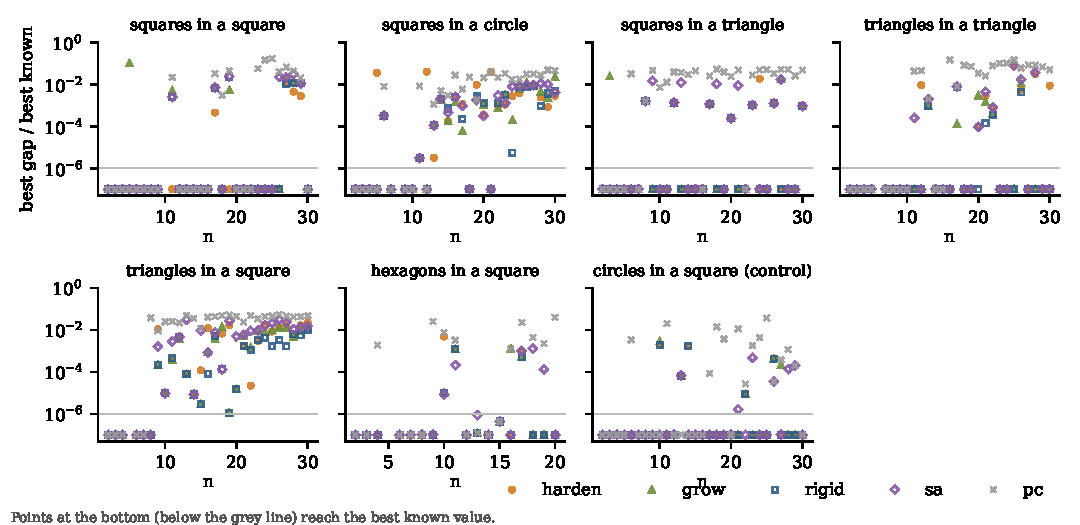
\includegraphics[width=\linewidth]{figures/gaps}
\caption{Lowest size reached per instance, relative to the best known value (C07). Points on the bottom row reach it.}\label{fig:gaps}
\end{figure}

\section{What we learned}\label{sec:learned}
\paragraph{The path matters, and which path depends on the family.} For squares in a square, hardening's lowest size is the lowest of all methods on \CsevenSquInSquHardenLowest{} of \CsevenSquInSquN{} instances and the only one that low on \CsevenSquInSquHardenSole{}; with identical settings, rigid starts manage \CsevenSquInSquRigidLowest{}. In 32 runs each, hardening alone reaches Trump's $n=11$ and Wainwright's $n=19$ packings (Figure~\ref{fig:strip}). For triangles the order reverses: rigid starts are lowest on \CsevenTriInSquRigidLowest{} instances of triangles in a square against \CsevenTriInSquHardenLowest{} for hardening, and \CsevenTriInTriRigidLowest{} against \CsevenTriInTriHardenLowest{} in a triangle (Figure~\ref{fig:tristrip}). On the control family the gradient paths reach the lowest size on the same number of instances, as they should.

\begin{figure}[t]\centering
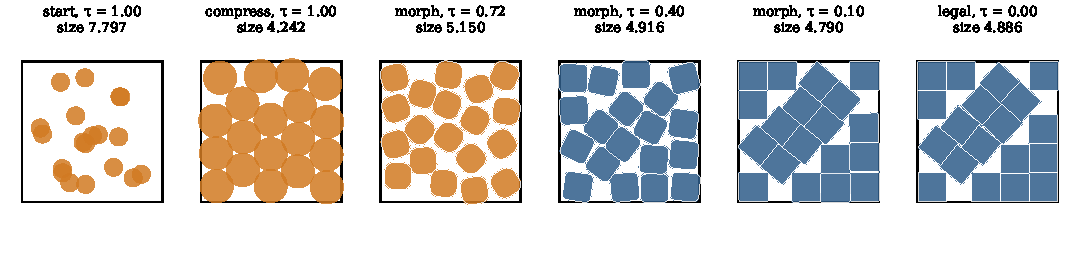
\includegraphics[width=\linewidth]{figures/strip_squ19}
\caption{One hardening run for 19 squares (C07): disks are compressed, harden into squares, and settle into Wainwright's packing (side $3+4\sqrt2/3$). Every replay is on the project site.}\label{fig:strip}
\end{figure}

\begin{figure}[t]\centering
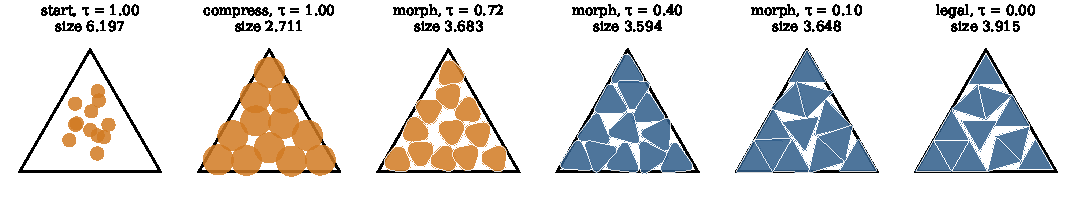
\includegraphics[width=\linewidth]{figures/strip_tri12}
\caption{The best of 32 hardening runs for 12 triangles in a triangle (C07) ends at $3.915$; rigid and snap starts reach the best known $3.879$. The disks settle into a near-hexagonal arrangement and the triangles that emerge from it keep orientations that do not tile.}\label{fig:tristrip}
\end{figure}

\paragraph{It is the gradual path, not the disk-compressed start.} Hardening differs from rigid starts in two ways: pieces are compressed as disks, and they then harden gradually. Campaign C11 separates the two with \emph{snap}, which compresses disks exactly as hardening does and then switches to the polygons in one step, with the same seeds, settings and budget (Table~\ref{tab:ablate}). We detect no difference between snap and rigid starts: over all \CsevenInstances{} instances each is lower than the other on \SnapRXLower{} and \SnapRRLower{} instances. Hardening differs from snap in both directions, by family: counting instances where hardening is lower against those where snap is lower, squares in a square give \SnapSquSqu{}, triangles in a triangle \SnapTriTri{} and triangles in a square \SnapTriSqu. The pre-registered test, over instances that exactly one of harden and snap solves, is \SnapHOnly{} against \SnapXOnly{} ($p=\SnapPReached$) over all families and inconclusive on squares in a square alone, where only two instances are discordant; the counts of lower sizes are clearer (harden \SnapHLower, snap \SnapXLower, $p=\SnapP$). The plan's rule says that if this test does not separate harden and snap on squares in a square, hardening's advantage there is attributed to the disk-compressed start. The test does not separate them, so that is the pre-registered conclusion; we record it, and also that the rule was poorly chosen, since a sign test over two discordant instances cannot reach significance. The rest of the evidence, which is descriptive and was not the pre-registered test, points the other way: we detect no gain from a disk-compressed start alone, and the instances where hardening and snap differ split by family, in hardening's favour on squares and against it on triangles.

\paragraph{Nor does the area schedule account for it.} A hardening piece also grows, by up to 40\% of its area. Campaign C12 keeps rigid polygons but scales them so that their area follows hardening's schedule exactly (\emph{grow-area}). We again detect no difference from rigid starts (lower on \AreaRXLower{} and \AreaRRLower{} instances, $p=\AreaRP$), and hardening differs from it in the same directions as from snap: \AreaSquSqu{} on squares in a square and \AreaTriTri{} on triangles in a triangle (Table~\ref{tab:ablate}). Over all instances, harden against grow-area is \AreaHLower{} against \AreaXLower{} ($p=\AreaP$); under the pre-registered rule (C12 uses C11's) the test on squares in a square is again inconclusive. Neither ablation reproduces hardening's pattern, which makes the rounding of the pieces the likeliest explanation, but these experiments do not establish it.

\begin{table}[t]\centering\small
\begin{tabular}{lrcccc}
\toprule
family & $N$ & harden : snap & snap : rigid & harden : grow-area & grow-area : rigid \\
\midrule
squares in square & 28 & 6 : 0 & 1 : 2 & 5 : 1 & 2 : 1 \\
squares in circle & 28 & 5 : 11 & 10 : 6 & 9 : 8 & 8 : 4 \\
squares in triangle & 29 & 0 : 1 & 0 : 0 & 0 : 1 & 0 : 0 \\
triangles in triangle & 28 & 0 : 8 & 0 : 2 & 1 : 8 & 0 : 3 \\
triangles in square & 28 & 6 : 14 & 8 : 9 & 5 : 11 & 5 : 6 \\
hexagons in square & 18 & 0 : 2 & 1 : 1 & 0 : 2 & 0 : 0 \\
disks in square & 29 & 0 : 0 & 0 : 0 & 0 : 0 & 0 : 0 \\
\midrule all & 188 & 17 : 36 & 20 : 20 & 20 : 31 & 15 : 14 \\
\bottomrule
\end{tabular}
\caption{Which part of hardening matters (C11, C12; harden and rigid from C07, same seeds, settings and budget). Each cell $a:b$ counts the instances on which the first method\textquotesingle s lowest size is lower than the second\textquotesingle s, and the reverse; the rest are ties. \emph{snap} compresses disks as hardening does, then switches to polygons at once; \emph{grow-area} keeps rigid polygons whose area follows hardening\textquotesingle s.}
\label{tab:ablate}
\end{table}


\paragraph{Why squares and not triangles?} We can only offer hypotheses. Along the path a piece's orientation matters in proportion to $1-\tau$ (Section~\ref{sec:method}), so hardening defers the choice of orientation until neighbours are nearly in place. Many of the best square packings, including $n=11$ and $19$, place a group of tilted squares between axis-aligned ones, where a late choice should help. The area explanation, that a triangle's inscribed disk covers only 60\% of it (a square's 79\%) and so a hardening triangle packing must grow and rearrange the most, is weakened by hexagons: their inscribed disk covers 91\%, yet hardening is no better than rigid starts there (lowest on \CsevenHexInSquHardenLowest{} against \CsevenHexInSquRigidLowest{} of \CsevenHexInSquN{} instances, mostly ties). A second hypothesis is orientational. Disks prefer a hexagonal arrangement; squares that emerge from it have four orientation classes and can tilt a little to fit, but good triangle packings alternate pieces pointing up and down, and a triangle's corners stick out twice as far as its inradius ($R/\rho=2$, against $\sqrt2$ for a square), so once corners appear a wrongly oriented triangle cannot turn without pushing its neighbours far apart. Figure~\ref{fig:tristrip} looks like this, but we did not test it.

\paragraph{Partly soft starts.} Varying only the starting softness $\tau_0$ on the \CtauN{} most contested instances (Table~\ref{tab:tau}), the counts of instances where each value reaches the lowest size are \CtauOne, \CtauHalf, \CtauQuarter{} and \CtauZero{} for $\tau_0=1, 0.5, 0.25, 0$. Squares in a square favour soft starts (\CtauSquares{}); triangles favour rigid or slightly rounded ones (\CtauTriangles{}). These instances were selected where hardening and rigid starts disagreed, mostly in rigid's favour, which tilts this count toward small $\tau_0$; partly rounded starts are a candidate default, not an established one.

\begin{table}[t]\centering\small
\begin{tabular}{lrrrrr}
\toprule
family & instances & $\tau_0=1$ (harden) & $0.5$ & $0.25$ & $0$ (rigid)\\
\midrule
squares in square & 6 & 3 & 4 & 2 & 0\\
squares in circle & 13 & 2 & 3 & 6 & 5\\
squares in triangle & 1 & 0 & 1 & 1 & 1\\
triangles in triangle & 7 & 0 & 4 & 3 & 5\\
triangles in square & 12 & 2 & 3 & 5 & 5\\
hexagons in square & 1 & 0 & 0 & 1 & 1\\
\midrule
all & 40 & 7 & 15 & 18 & 17\\
\bottomrule
\end{tabular}
\caption{How soft the start must be (C08): on the 40 most contested instances of C07, the number of instances where each starting softness $\tau_0$ reaches the lowest size (32 runs each, all other settings equal; ties counted for every tied value).}
\label{tab:tau}
\end{table}


\paragraph{Longer runs, or more runs?} An earlier test (C09, appendix) suggested that hardening gains more than rigid starts from longer schedules, but it changed run length and restart count together and used instances chosen because the two paths disagreed. Campaign C13 repeats it cleanly on \BudN{} instances fixed in advance ($n=11,17,23,29$ per family; hexagons $n=8,12,16,20$), with 32 runs at three times the budget, and 96 runs at the base budget for the same total cost. Counting instances where hardening is lower against those where rigid starts are lower: \BudOneH{} against \BudOneR{} with 32 base runs ($p=\BudOneP$), \BudThreeH{} against \BudThreeR{} with 32 long runs, and \BudMoreH{} against \BudMoreR{} with 96 base runs. Longer runs improved rigid starts more than hardening (rigid lower than its base on \BudGainR{} instances and higher on \BudLossR; hardening \BudGainH{} and \BudLossH), and at equal cost, three times longer runs and three times as many runs did about equally well for both paths (\BudLvMLH{} against \BudLvMMH{} for hardening, \BudLvMLR{} against \BudLvMMR{} for rigid). The C09 result does not replicate; we withdraw it.

\paragraph{Two paths, or more runs of one?} The paths fail on different families, so running both might help. At equal total budget, 32 rigid runs plus 32 hardening runs solve \PortRigidHarden{} of the \CsevenInstances{} instances, against \PortRigidSixtyFour{} for 64 rigid runs and \PortRigidGrow{} for 32 rigid plus 32 growing runs (instances solved by exactly one of the first two: \PortSign, two-sided $p=\PortP$). We detected no benefit from mixing; at this size that does not show there is none, and whether mixing pays when the family is known to favour the second path was not tested.

\paragraph{Tuning decides comparisons.} Our first experiments compared hardening with rigid starts that inherited the hardening schedule, on two square instances, and hardening looked better. Tuned with comparable effort, rigid starts led overall. Re-tuning for the lowest point instead of the median changed four of the five methods' settings (stronger pressure for the gradient paths, more noise for rigid starts) and helped simulated annealing most. It kept the broad pattern, hardening for squares in a square and rigid or growing starts for triangles, though the leading method changed for squares in a circle and triangles in a square.

\section{Downstream use and where to rerun the protocol}\label{sec:matters}
\paragraph{Downstream use.} The earlier cube release \cite{softtorigidpacking} has been reused by others; we report this separately from our results, which it does not change. A continuation of the unfinished $n=13$ cube search \cite{n13repo} reuses our simulator, tightening code and checkers unchanged, adds two moves (re-melting a finished packing: soften, expand slightly, reharden; and inserting a thirteenth cube into the 12-cube packing), and after 2{,}627 runs reports a certified packing of side $2.956149$ at $10^{-6}$ clearance, consistent with Friedman's $2.956+$ and not claimed as an improvement; our C05 reaches the same value. Zarzuelo \cite{platonicrepo} generalises the construction to all five Platonic solids as pieces and containers, with exact feasibility checks over $\mathbb{Q}(\sqrt2,\sqrt5)$ and an archive search that repeatedly softens and rehardens existing packings; the reported values are certified upper bounds, and comparisons with Berthold et al.\ \cite{Berthold2026} must convert between edge and circumradius normalisations. Yudhiono \cite{tesseractrepo} reimplements ball-to-hypercube continuation independently in four dimensions and combines it with structured seeds, constrained polishing and basin hopping, reporting floating-point candidates for 26--30 tesseracts. None of these is a controlled comparison, and only the last is an independent implementation; the other two build on our simulator and checkers, so they are not independent validations. What they add is a use we did not test: softening as a rearrangement operator inside a larger search rather than only as a cold start. Whether temporary softening escapes a rigid local optimum better than rigid perturbation at equal budget, from shared starting packings, is the experiment they motivate.

\paragraph{Other settings.} The same question arises wherever an overlap penalty is minimised in a shrinking container: irregular nesting \cite{Wascher2007,Bennell2008,Leao2020}, where inscribed circles are already an overlap proxy \cite{Jones2014,Gardeyn2025}; floorplanning, where circles-then-rectangles is an established two-stage switch \cite{AnjosVannelli2002,Luo2008}; and faceted particles in confinement \cite{Torquato2018,Wang2018}. In each, C11 is the test to run first, and real objectives add stability, orientation and ordering constraints \cite{Bortfeldt2013,Araujo2019} that any gain in density must survive.

\section{Limitations and open directions}\label{sec:limits}
\paragraph{Limitations.} These are search results, not optimality proofs, and tightening is a local method. In the main comparison (C07) each instance had 32 runs per method at a fixed budget, and C16 had 16; the $n=12$ cube record came from one of 192 runs, and ``only one method reached it'' holds within the run count and budget stated for that campaign. Gradient paths are matched in steps, not pair evaluations or wall-clock time (hardening was the fastest per run on polygon families); the baselines are matched to a hardening run's pair evaluations, which perturbation--compression overshoots (Table~\ref{tab:diag}). Simulated annealing and perturbation--compression are our implementations; their best runs were less often close enough to be tightened, so the tightening policy favours the gradient paths, most for pc (C14 shows the order survives equal tightening on 28 instances); in C16 the other methods' best runs at the hardening-only instances were tightened after the fact and remained short of the best known value. The lowest-point tuning used instances larger than the test set, and in that round every winner sat on a grid edge or corner and, as pre-registered, the grid was not extended. In 3D only the three gradient paths were compared. Catalogue values come from captions and witnesses as of October 2026; truncated values are only known to their printed precision. Not detecting a difference (between mixed and single-path portfolios, between snap or grow-area and rigid starts, or between the pilot and always-rigid) is not evidence of equivalence at these sample sizes.

\paragraph{Open directions.}
\begin{itemize}\itemsep1pt
\item \emph{A rule that predicts the path.} The pilot showed no detected benefit on held-out families that had no aggregate hardening advantage. A useful rule would have to predict, before running, the families where it does; we have one such family and no rule that singles it out in advance.
\item \emph{External baselines.} Our simulated annealing and perturbation--compression are our own implementations. Running a published nester \cite{Gardeyn2025} or solver \cite{Berthold2026} once, untouched, at the same budget would test whether they were given a fair fight.
\item \emph{Softening as a move.} Re-softening an existing packing and rehardening it, as downstream searches do \cite{n13repo,platonicrepo}, against rigid perturbation from the same packings at equal budget.
\item \emph{Other paths.} Paths through other shape families (an ellipse for a rectangle, a rounded octahedron for a cube, superellipses \cite{Jiao2008}), paths that harden pieces one at a time, or schedules that adapt $\tau$ to the current overlap.
\item \emph{Larger $n$, other solids, other solvers.} Most unsolved instances have $n\ge17$. Our controlled study did not include solids other than cubes; downstream work now explores them \cite{platonicrepo} and higher dimensions \cite{tesseractrepo}, without controlled baselines. Hardening could also seed exact models \cite{Berthold2026} or shrink-and-separate nesters \cite{Gardeyn2025}.
\item \emph{Non-convex and mixed pieces.} The rounded-shape construction needs a convex core; non-convex pieces would need a different family of intermediate shapes, for example a convex decomposition hardened part by part.
\end{itemize}



\sloppy
\paragraph{Reproducibility.} Every run, replay, certificate and decision is in the repository \url{https://github.com/yoheinakajima/soft-to-rigid} and its site, \url{https://yoheinakajima.github.io/soft-to-rigid/}. Each experiment was planned in writing before it ran; the plans, the raw results and the research ledger (an ActiveGraph event log \cite{activegraph}) are committed, and every number in this paper is generated from the ledger.

\paragraph{Acknowledgements.} Code, experiments and verification were developed with Claude (Anthropic), an AI system, under the author's direction. The author takes responsibility for the content.

\FloatBarrier
\bibliographystyle{abbrvnat}
\setlength{\bibsep}{1pt plus 0.3ex}
\renewcommand{\bibfont}{\footnotesize}
\bibliography{refs}

\appendix
\section{Supplementary tables}
\begin{table}[t]\centering\small
\begin{tabular}{lrccccc}
\toprule
family & $N$ & \textbf{harden} & \textbf{grow} & \textbf{rigid} & \textbf{sa} & \textbf{pc} \\
\midrule
squares in square & 28 & \textbf{28 (7)} & 21 & 20 & 10 & 17 \\
squares in circle & 28 & 16 (7) & 11 (2) & \textbf{19 (9)} & 10 & 8 \\
squares in triangle & 29 & 27 & 24 & \textbf{29 (1)} & 13 & 7 \\
triangles in triangle & 28 & 19 (1) & 22 (3) & \textbf{24 (4)} & 8 & 10 \\
triangles in square & 28 & 10 (1) & \textbf{19 (5)} & 18 (7) & 12 (1) & 5 \\
hexagons in square & 18 & 15 & 15 (1) & \textbf{17 (2)} & 8 & 6 \\
circles in square (control) & 29 & 27 & 27 & \textbf{28} & 11 (1) & 11 \\
\midrule
all & 188 & 142 (16) & 139 (11) & \textbf{155 (23)} & 72 (2) & 64 (0) \\
reached best known & & 121 & 119 & 132 & 69 & 63 \\
\bottomrule
\end{tabular}
\caption{Settings tuned by median gap (C04). Same layout as Table~\ref{tab:main}.}
\label{tab:median}
\end{table}


\paragraph{Frozen settings.} Median-tuned (C01--C03): harden $\mu=0.08$, noise $\times8$; grow $\mu=0.04$, $\gamma_0=0.2$; rigid $\mu=0.04$, noise $\times2$; sa $T_0=3\cdot10^{-3}$, $\mu=0.0025$; pc kick $0.05$, relax $19200$ steps. Lowest-point-tuned (C06): harden and rigid $\mu=0.16$, noise $\times8$; grow $\mu=0.08$, $\gamma_0=0.1$; sa $T_0=10^{-3}$, $\mu=0.02$; pc kick $0.05$, relax $19200$ steps. All are in \texttt{methods/*.json}, each with the campaign and grid point that selected it.

\paragraph{Campaigns.} C00 reproduce the earlier square results; C01--C03 median tuning; C04 breadth (median-tuned); C05 cubes; C06 lowest-point tuning; C07 breadth (lowest-point-tuned, main); C08 starting softness; C09 longer schedules; C10 portfolio. Plans, amendments, raw runs, reports and the decision recorded for each are in \texttt{campaigns/} and the journal.

\end{document}
